% !TEX root = ../main.tex

% 中英标题:\chapter{中文标题}[英文标题]
\chapter{绪\ 论}[Introduction]

\section{课题背景及研究的目的和意义}[Background, objective and significance of the subject]

% 正文内容,注意LaTeX分段有两种方法,直接空一行或者使用<\par>
% 默认首行缩进,不需要在代码编辑区手动敲空格
\subsection{课题背景}
近些年来,随着控制科学、感知导航以及人工智能等技术的不断进步,关于多旋翼无人机(multirotor UAV)的设计及应用的领域展现出了空前的繁荣,并取得了长足的发展。
多旋翼无人机凭借其简洁的机械结构以及优秀的飞行稳定性,从一众智能机器人中脱颖而出,从实验室里走进了千家万户。
在许多地方,如日常生活中的航拍,或是农林、检修和军事行动等特种作业场合中,都有多旋翼无人机的用武之地(\figref{fig:applications})。

\begin{figure}[!ht]
    \setlength{\subfigcapskip}{-1bp}
    \centering
    \begin{minipage}{\textwidth}

    \centering
    \subfigure{\label{fig:aerial_photo}}\addtocounter{subfigure}{-2}
    \subfigure{\subfigure[用于航拍测绘]{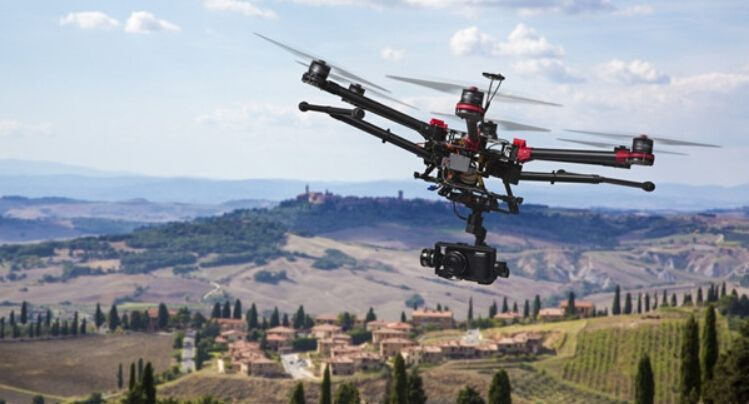
\includegraphics[width=0.45\textwidth, height=0.25\textwidth]{aerial_photo.jpeg}}}
    \hspace{0.2em}
    \subfigure{\label{fig:farming}}\addtocounter{subfigure}{-2}
    \subfigure{\subfigure[用于农林植保]{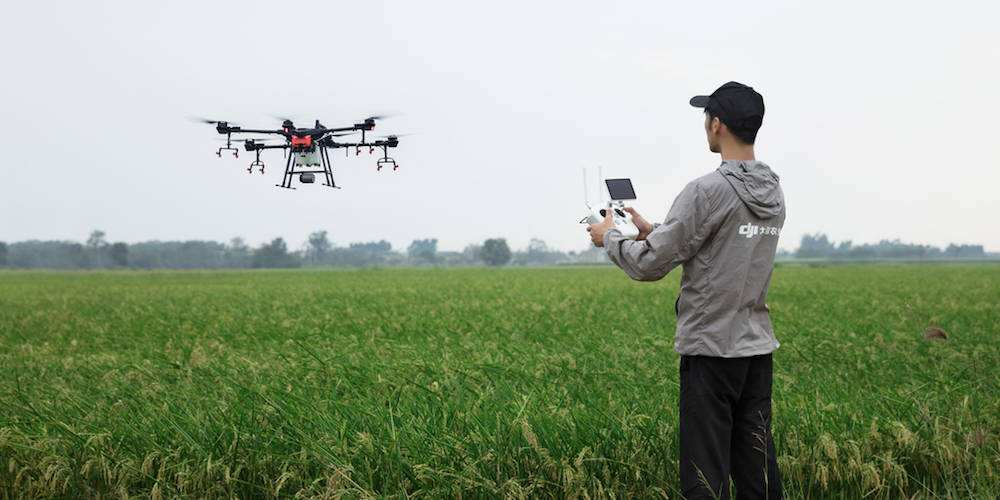
\includegraphics[width=0.45\textwidth, height=0.25\textwidth]{farming.jpeg}}}

    \subfigure{\label{fig:inspection}}\addtocounter{subfigure}{-2}
    \subfigure{\subfigure[用于电力巡检]{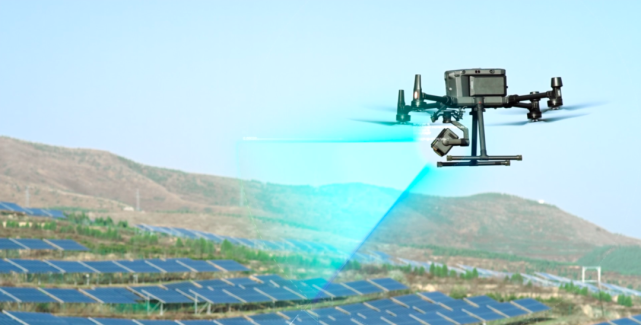
\includegraphics[width=0.45\textwidth, height=0.25\textwidth]{inspection.jpeg}}}
    \hspace{0.2em}
    \subfigure{\label{fig:logistics}}\addtocounter{subfigure}{-2}
    \subfigure{\subfigure[用于后勤补给]{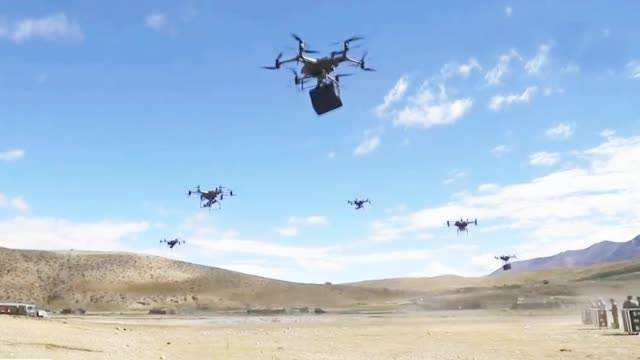
\includegraphics[width=0.45\textwidth, height=0.25\textwidth]{logistics.jpeg}}}
    
    \end{minipage}
    \caption{多旋翼无人机的多种应用场景}
    \label{fig:applications}
\end{figure}

然而,从机械结构中可以发现,目前所应用的大多数多旋翼无人机的各个旋翼的转轴均互相平行且垂直于机身平面,所以旋翼只能为飞行器提供垂直机身平面的推力。
这就使得飞行器成为一个欠驱动系统(under-actuated system)\cite{2012Underactuated},其位置控制和姿态控制是耦合的。
具体表现为,如果飞行器需要水平飞行,则必须倾斜机身才能获得水平方向的分力,以提供水平方向的加速度和克服空气阻力;
类似地,飞行器只有在水平姿态下才可以保持悬停。
这种特性很大程度上限制了欠驱动多旋翼飞行器的应用场景:
在空中作业时,悬停姿态的限制会使飞行器无法克服机载机械臂或机载云台的机械死角;
在拥挤的环境中,姿态与推力的耦合也会严重削弱飞行器的避障性能,使环境中的可行区域大幅缩减。

为了改善上述问题,充分发掘多旋翼飞行器的潜力,近年来发展出了多种能将飞机的位置与姿态控制解耦的多旋翼飞行器。
这些工作通过改变旋翼几何构型、增加旋翼倾转自由度等方式让旋翼能提供相对机身任意方向的推力和转矩,这赋予了多旋翼飞行器跟踪6自由度全状态轨迹的能力,使飞行器成为全驱动系统(fully actuated system)。
这种飞行器能够分别独立地进行平移和旋转运动,故又称为全向飞行器(omnidirectional aerial vehicle),这种受控的、自由的刚体运动是传统欠驱动多旋翼飞行器所无法做到的。
所谓过驱动飞行器,就是具有冗余控制输入(驱动器)的全驱动飞行器,在少数驱动器故障的情况下依然能够进行控制,增强了飞行器的容错能力。


\subsection{研究的目的和意义}
由于上述过驱动多旋翼飞行器的位置和姿态可以独立控制,故可以为其独立规划位置和姿态共6个自由度的轨迹,其飞行的灵活性相比于只能跟踪4自由度轨迹的传统欠驱动多旋翼飞行器将大幅提高。
设想当面对一个狭长笔直、宽度小于自身旋翼间最小距离的通道时,加速度与姿态耦合的欠驱动飞行器显然无法通过;
而过驱动飞行器则可以通过控制姿态使机身倾斜以适应通道内的狭小空间,同时控制位置从而实现平稳无碰撞的穿越。
这样的优势使得过驱动飞行器在未知环境探索、巷战侦查与打击、灾区废墟搜救等场合势必会发挥出很大的应用价值。
要更好地挖掘过驱动多旋翼飞行器的潜力,提高其自主飞行性能,那么为其设计一套在复杂狭小空间内进行避障轨迹规划的算法是具有重要意义的。

本文以实现过驱动多旋翼飞行器在复杂环境中的避障飞行为目标,对基于过驱动多旋翼飞行器的SE(3)运动规划算法展开研究,设计了一个考虑飞行器整体形状和动力学约束的全局轨迹规划器,
并设计仿真和实物实验验证了所设计规划器的可行性,为相关领域探索了一条可行的道路,且有望后续通过并行计算及对算法进行优化等手段,配合机载感知系统实现实时规划。


\section{国内外研究现状}[Developmental of gas-lubricated bearing and correlated theories]
轨迹规划模块处于无人机软件框架的中间位置,其接收感知模块传来的地图等上游信息,输出一条安全、平滑的可行轨迹输送给控制模块。
规划模块起到了承上启下的作用,可以说是影响无人机自主飞行性能的最重要的一环;
另外,在多旋翼飞行器全驱动化方面,目前也有不少种方案可以参考。
本节将从欠驱动多旋翼飞行器的避障轨迹规划、过驱动多旋翼飞行器和过驱动多旋翼飞行器的轨迹规划三方面讲述国内外研究现状。

\subsection{欠驱动多旋翼飞行器的避障轨迹规划}
多旋翼飞行器的避障轨迹规划这一领域近年来取得了丰富的成果。
大多数多旋翼飞行器属于微分平坦系统\cite{2003Flatness},这种系统的运动规划问题可以在保证一定的平滑性的前提下转化为较低维度的优化问题。
其轨迹可以表示为分段多项式,这样就能方便地获得轨迹关于时间的各阶导数,进而利用微分平坦关系求得飞行器的各状态变量和控制输入。

2011年,Mellinger等人提出了为四旋翼飞行器生成固定间隔多项式轨迹的方法\cite{2011minimumsnap},通过求解一个由加速度的二阶导数(即snap)的平方积分代价以及线性安全约束构造的二次规划(Quadratic Programming,QP)问题,最终生成一条平滑且安全的轨迹。
2015年,Bry等人推导出了导数平方积分形式无约束二次规划问题的闭式解\cite{bry2015aggressive},并且启发式地在前端RRT*搜索出的可行路径上添加路点直到无碰撞为止,以此来保证轨迹的安全性。
2020年,Gao等人将环境中的安全区域表示为凸多面体\cite{gao2020teach},一系列凸多面体连接起来构成安全飞行走廊(safe flight corridor,SFC)(\figref{fig:TTR}),轨迹的安全性由B\'{e}zier曲线的凸包性质来保证。
\begin{figure}[!ht]
    \setlength{\subfigcapskip}{-1bp}
    \centering
    \begin{minipage}{\textwidth}

    \centering
    \subfigure{\label{fig:ttr_corridor}}\addtocounter{subfigure}{-2}
    \subfigure{\subfigure[生成的安全飞行走廊]{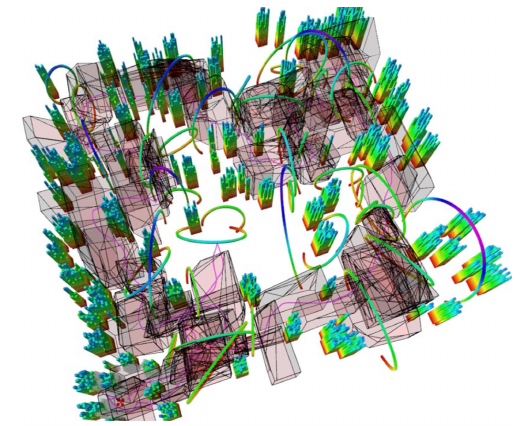
\includegraphics[width=0.4\textwidth, height=0.4\textwidth]{gao2020teach_a.png}}}
    \hspace{0.2em}
    \subfigure{\label{fig:ttr_trajectory}}\addtocounter{subfigure}{-2}
    \subfigure{\subfigure[经过优化的轨迹]{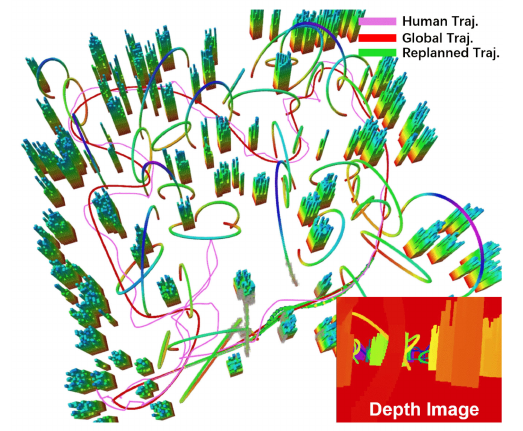
\includegraphics[width=0.4\textwidth, height=0.4\textwidth]{gao2020teach_b.png}}}
    
    \end{minipage}
    \caption{Teach-Repeat-Replan示意图\cite{gao2020teach}}
    \label{fig:TTR}
\end{figure}
2021年,Zhou等人提出了EGO-Planner,与多数基于梯度的轨迹规划方法不同,EGO-Planner直接从障碍物上获得梯度信息,从而免去了对ESDF地图的依赖,大大降低了内存消耗和计算量。

\begin{figure}[ht]
    \centering
    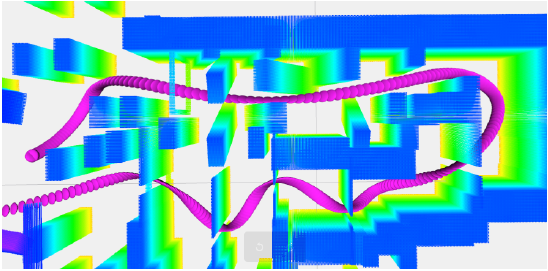
\includegraphics[width = 0.65\textwidth]{se3_traj.png}
    \caption{在SE(3)空间中规划出的轨迹\cite{2021Fast}}
    \label{fig:se3_traj}
\end{figure}

以上工作都能高效地进行轨迹规划,然而它们都是在构型空间(configuration space)中进行规划,并未考虑无人机的几何形状和姿态,具有很大的保守性。
在某些比较极端的环境中,存在需要无人机倾斜机身才能飞过的狭窄缝隙,此时传统的$\mathbb{R}^3$规划器是难以发挥作用的。
要得到如\figref{fig:se3_traj}所示通过改变姿态在较为拥挤的环境中的安全轨迹,就需要在SE(3)空间中进行规划。
2018年,Liu等人提出了一种基于搜索的SE(3)规划算法\cite{liu2018search},其通过在一定的时间间隔内施加常量控制输入来生成运动基元(motion primitive),配合可行性检测器筛选出与点云无交集的运动基元,最终搜索出一条无碰撞轨迹。
不过,该算法存在着组合爆炸(combinatorial explosion)问题:要想获得更高的求解质量,就得提高分辨率,而随着分辨率的增高,计算量会快速增加,带来不可接受的计算时间和内存消耗,故这种算法实用性欠佳。

2022年,Wang等人提出了一个几何约束下的多旋翼飞行器轨迹优化框架\cite{wang2022geometrically}。该框架首先基于多阶段最优控制问题的最优充要条件,构建了名为MINCO的一类分段多项式轨迹,这类轨迹以其必须经过的中间点和每段的时间分配作为参数,轨迹的系数矩阵可以根据最优条件以线性的时间和空间复杂度计算出来,这相较Bry等人提出的闭式解\cite{bry2015aggressive}有了很大改进;
使用MINCO轨迹类,就可以直接对中间点和时间分配进行优化,同时还能保证轨迹的平滑性。
该框架还通过一系列技巧消去了对时间分配的约束以及中间点的空间约束,并将其余自定义约束软化为目标函数中的惩罚项,最终将整个带约束的轨迹优化问题转化为无约束优化问题,得以高效求解。
该框架的提出为SE(3)规划问题提供了新思路,紧接着Yang等人构造了考虑四旋翼飞行器的形状与姿态,并使飞行器整体包含在表示安全区域的凸多面体内的约束形式\cite{yang2021whole},该约束作为框架中的自定义约束来处理;Han等人进一步开发了用于无人机竞速的SE(3)规划器\cite{2021Fast},并将其开源\footnote{https://github.com/ZJU-FAST-Lab/Fast-Racing}。


\subsection{过驱动多旋翼飞行器}[Developmental of gas-lubricated bearing]
实现多旋翼飞行器全驱动化的要点在于使驱动器同时且独立地产生相对机体任意方向推力和力矩,而要做到这一点需要改变旋翼的构型(configuration of rotors)。
过驱动全向多旋翼飞行器领域近年来正处于持续发展中,这些全向飞行器按照旋翼构型大致可分为两类:固定旋翼型(fixed-rotor)\cite{brescianini2016design, park2018odar,allenspach2020design}和倾转旋翼型(tiltrotor)\cite{ryll2014novel, kamel2018voliro,2021Geometrically}。
\figref{fig:omav}分别展示了两种构型中具有代表性的一项工作。

\begin{figure}[!ht]
    \setlength{\subfigcapskip}{-1bp}
    \centering
    \begin{minipage}{\textwidth}

    \centering
    \subfigure{\label{fig:omav_1}}\addtocounter{subfigure}{-2}
    \subfigure{\subfigure[固定旋翼型\cite{brescianini2016design}]{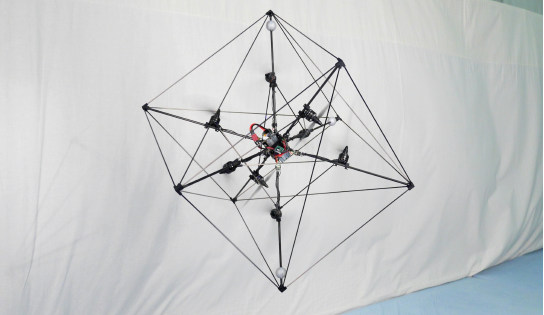
\includegraphics[width=0.4\textwidth]{octo_omav.png}}}
    \hspace{0.2em}
    \subfigure{\label{fig:omav_2}}\addtocounter{subfigure}{-2}
    \subfigure{\subfigure[可倾转旋翼型\cite{kamel2018voliro}]{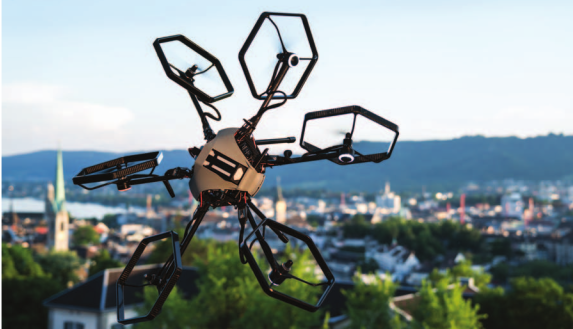
\includegraphics[width=0.4\textwidth]{voliro_2.png}}}
    
    \end{minipage}
    \caption{两种不同种类旋翼构型的全向多旋翼飞行器示例\label{fig:omav}}
\end{figure}

固定旋翼的过(全)多旋翼飞行器的机械结构相对简单,飞行器通过改变不同朝向旋翼的转速来控制推力和转矩的大小和方向。
如\figref{fig:omav_1}所示为Brescianini等人于2016年发表的一种实现灵活全向飞行的固定旋翼型八旋翼飞行器系统\cite{brescianini2016design},
该系统采用8个可逆电机-旋翼组合执行器(reversible motor-propeller actuator),故每个执行器都可以产生正推力和负推力,
8个执行器的构型是基于静态力和扭矩分析,采用求解优化问题的方式来设计的,以期最大化飞行器的灵活性并最大限度保证飞行器动力学特性的旋转不变性。
不过,固定旋翼型的过驱动飞行器的一个主要缺点在于:这些旋翼通常不会同时直接朝向竖直方向,使得这类飞行器的悬停效率不会很高;
并且如果设定旋翼朝向使之更倾向于高效的悬停和更高的有效载荷,就会几乎不可避免地降低产生横向作用力的能力\cite{allenspach2020design}。

可倾转旋翼型全向多旋翼飞行器的实现方式多数是为旋翼增加额外的自由度,使其转轴指向可以改变。
比较常用的方式是为安装旋翼的机臂添加一个绕其轴的旋转自由度:
如\figref{fig:tiltrotor_quadrotor}展示了Markus等人于2015年研制出的一种可倾转旋翼的过驱动四旋翼飞行器的结构\cite{ryll2014novel},该飞行器可以在有限的横滚角和俯仰角下实现悬停;
\figref{fig:omav_2}展示的是Kamel等人于2018年开发的一种可倾转旋翼的全向六旋翼飞行器Voliro\cite{kamel2018voliro},该飞行器可以实现任意姿态下的悬停和飞行。
这类飞行器通过改变每个旋翼的朝向,实现了更高效的悬停。
本课题所使用的仿真及实物实验平台是参考Voliro的结构搭建的。

\begin{figure}[ht]
    \centering
    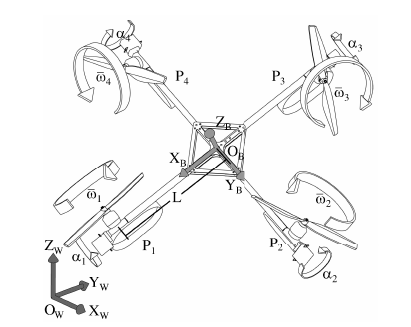
\includegraphics[width = 0.65\textwidth]{omni_quadrotor.png}
    \caption{Markus Ryll等人的可倾转旋翼的全向四旋翼飞行器结构示意图}
    \label{fig:tiltrotor_quadrotor}
\end{figure}

\subsection{过驱动飞行器的轨迹规划}
现有的关于过(全)驱动飞行器的研究主要集中于机械结构设计和飞行控制算法方面,而为过驱动飞行器进行轨迹规划的相关成果并不太多。
2018年,Brescianini等人基于运动基元为过驱动飞行器生成了从给定起点到给定终点且满足一定动力学约束的6自由度轨迹\cite{brescianini2018computationally}。
同年,Morbidi等人提出了用于双轴倾转旋翼六旋翼飞行器的节能轨迹生成方法\cite{morbidi2018energy},通过求解一个显式考虑电机电气模型的优化控制问题得到一条指定边界点的节能轨迹,并做了数值验证。
2021年,Pantic等人提出了基于流形网格的运动规划方法\cite{pantic2021mesh},该方法将物体表面(surface)建模为三角网格(triangular mesh)并提出原始表面的一个低维参数化表示方法,进一步将原始表面及其低维表示近似为流形(manifold),运用黎曼运动策略(Riemannian Motion Policies,RMPs)构建了一个高效且通用的运动规划框架;
该方法目的在于生成一条使飞行器飞向指定表面并沿其飞行,应用于全向飞行器与曲面交互的场景。

\section{本文的主要研究内容}[Main research contents of this subject]
从国内外研究现状中可以看出,目前已有许多成熟的方案能赋予多旋翼无人机跟踪6自由度轨迹、实现全向飞行的能力。
在避障轨迹规划方面,以欠驱动多旋翼飞行器为平台的解决方案同样多样且成熟,其中在复杂空间内进行SE(3)避障规划也已经有了效果拔群的成果;
然而,在能够进行全向飞行的过驱动多旋翼飞行器平台上进行轨迹规划的成果并不多,其中多数\cite{brescianini2018computationally, morbidi2018energy}并未考虑障碍物存在情况下的安全约束,Pantic等人的方法\cite{pantic2021mesh}也并不太适用于避障。
事实上,面向复杂环境中过驱动飞行器的SE(3)轨迹规划的解决方案还未见已发表的成果。
传统基于欠驱动多旋翼飞行器的轨迹规划方法固然可以应用到过驱动飞行器上,但由于这些方法并不能生成6自由度轨迹,所以它们并不能充分发挥过驱动飞行器的避障潜能。

本文重点研究过驱动多旋翼飞行器在复杂环境中的SE(3)轨迹规划。
通过深入研究、对比各种已有的轨迹规划方案,结合过驱动飞行器的不同性质,完成规划算法设计、代码实现、仿真验证及实物验证。
本文主要研究内容如下:
\begin{enumerate}
    \renewcommand{\labelenumi}{(\theenumi)}
    \item 参考过驱动飞行器系统Voliro\cite{kamel2018voliro},搭建了全向六旋翼飞行器OmniHex的仿真和实物模型,并对其动力学模型进行研究和分析。
    \item 针对前端路径搜索和安全飞行走廊生成的问题,研究已有方案和开源代码,设计SE(3)空间中的RRT算法用于前端路径搜索,设计凸多面体安全飞行走廊生成算法用于空间约束的生成。
    \item 为实现复杂环境中的6自由度SE(3)轨迹规划,对姿态规划方式及后端轨迹优化问题展开研究,设计了基于欧拉角和基于四元数的两种姿态规划方式,并分别设计对应的安全约束和动力学约束形式,推导对应的罚函数及其梯度。
    \item 将所设计的算法实现为C++接口,并对其进行整合,实现为基于ROS\cite{quigley2009ros}的全局规划器,并基于Gazebo\cite{gazebo}和PX4\cite{meier2015px4}进行仿真实验、基于实物平台进行实物实验验证其可行性。
\end{enumerate}

